
\chapter{Projekt: Udvidelse af \emph{photon mapping}}
\label{cha:project}

I vores projekt valgte vi at udvide raytraceren til underst�tte den
fulde \emph{photon map}-algoritme. Derudover har vi implementeret
firkantede \emph{area lights}.

\section{Area lights}
\label{sec:area-lights}

\emph{Area lights} er lyskilder, der har en st�rrelse. Derudover
udsender de ikke lys i alle retninger, men kun i en forudbestemt
retning (dvs. ligesom en ``normal'' loftslampe i virkeligheden).

En af ``sideeffekterne'' ved at bruge \emph{area lights} er, at
skygger bliver bl�de, da et punkt kan v�re v�re belyst af en del af
lampen i stedet for enten at v�re i fuldkommen skygge eller fuldkommen
lys.

\emph{Arealights} er inddelt i et antal \emph{sample}punkter, fordel
over hele overfladen. N�r der \emph{traces}, skal hvert punkt
unders�ge om det ligger i lys �n gang for hvert \emph{sample}punkt p�
lyskilden. Det g�r naturligvis, at renderingstiden for�ges, men
billedkvaliteten for�ges ogs�, idet skygger og lyseffekter bliver mere
realistiske.

[ figur ]

Ligeledes skal der ved fotonudsendelse udsendes lige mange fotoner fra
alle \emph{samples}. Dette g�res ved at udsende �n foton fra f�rste
samplepunkt, �n foton fra n�ste samplepunkt og s� fremdeles til alle
samplepunkter er bes�gt, hvorefter der startes forfra.

For simplicitetens skyld, underst�tter vi kun firkantede
\emph{arealights}.

Vores scene renderet med \emph{photon mapping} og et \emph{area light}
i stedet for et punktlys kan ses p� figur
\ref{fig:arealights_all}. Bem�rk, at \emph{ambient}-lys er fjernet fra
scenen.

\begin{figure}[htbp]
  \centering
  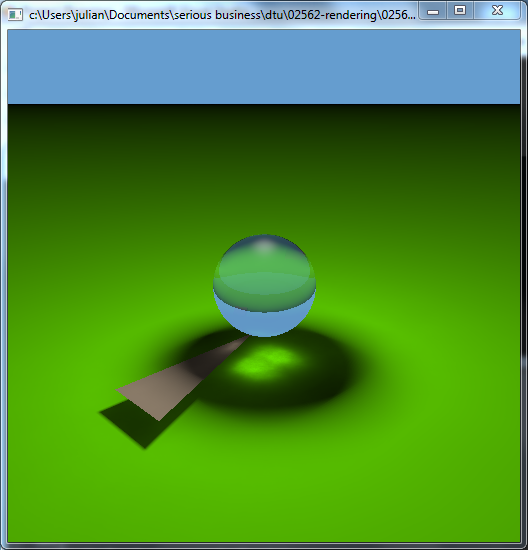
\includegraphics[width=8cm]{screenshots/project/01-arealights_with_all.png}
  \caption{\emph{Arealights} tilf�jet vores raytracer fra ugeopgave 9}
  \label{fig:arealights_all}
\end{figure}

\section{Den fulde \emph{photon mapping} algoritme}
\label{sec:den-fulde-photon}

Trinnet, der manglede fra for at have implementeret den fulde \emph{photon
map}-algoritme, var \emph{final gather}. \emph{Final gather} er at
erstatte opslaget i \emph{photon mappet} ved det f�rste \emph{ray}-hit
med en Monte Carlo-integration af det indirekte diffuse lys i punktet.

Dette har vi gjort ved at udsende en reflekteret str�le fra
hit-punktet og sl� op i \emph{photon mappet} hvis den reflekterede
str�le ramte et andet objekt. Opslaget blev lavet med en st�rre radius
end et normalt opslag. Dette sker, for at erstatte h�jfrekvens-st�j i
\emph{photon mappet} med lavfrekvens-st�j fra ``integrationen''. Det
tillader os at udsende f�rre fotoner og samtidig opn� en visuel
kvalitet der stadig er god. Ulempen ved dette er, at \emph{caustics}
samt direkte lys forsvinder. Det direkte lys kan dog simpelt gendannes
vha. den normale raytracing-metode. En rendering foretaget med $1000$
fotoner uden \emph{final gather} kan ses p� figur
\ref{fig:1000_no_final_gather} mens en rendering med $1000$ fotoner og
\emph{final gather} kan ses p� figur \ref{fig:1000_final_gather}.

\begin{figure}[htbp]
  \centering
  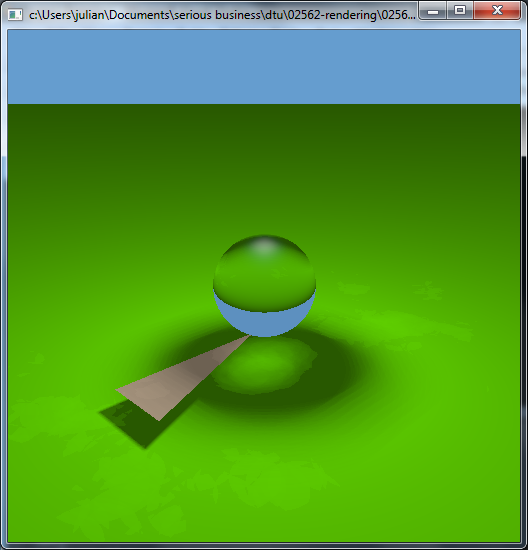
\includegraphics[width=8cm]{screenshots/project/02-1000_photons.png}
  \caption{1000 fotoner uden \emph{final gather}}
  \label{fig:1000_no_final_gather}
\end{figure}

\begin{figure}[htbp]
  \centering
  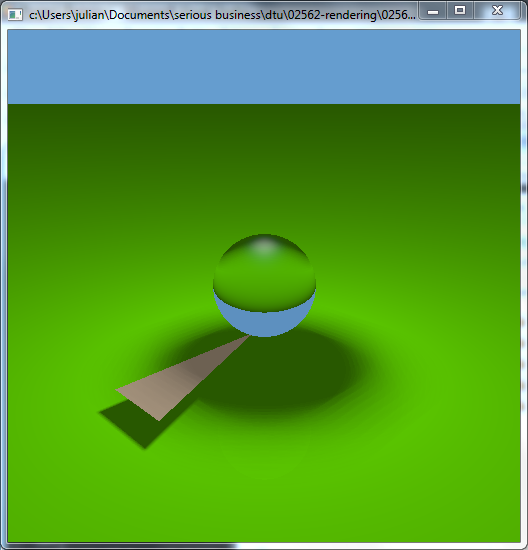
\includegraphics[width=8cm]{screenshots/project/03-1000_photons_final_gather.png}
  \caption{1000 fotoner med \emph{final gather}}
  \label{fig:1000_final_gather}
\end{figure}

\subsection{Gendannelse af \emph{caustics}}
\label{sec:gend-af-caust}

For at f� \emph{caustics} til at vise sig p� det renderede billede
igen, skal der genereres et seperat \emph{caustic photon map}. Dette
g�res ved kun at gemme de fotoner, der har v�ret igennem en
$L~S^+~D$-vej. Samtidig skal man s�rge for at disse fotonveje ikke
gemmes i det normale \emph{photon map}. N�r \emph{tracingen}
foretages, laves der et opslag i \emph{caustic photon mappet} og
resultatet herfra bruges sammen med de �vrige bidrag til at bestemme
den endelige farve.

Resultatet af det seperate \emph{caustic photon map} kan ses p� figur
\ref{fig:caustic_photon_map}.

\begin{figure}[htbp]
  \centering
  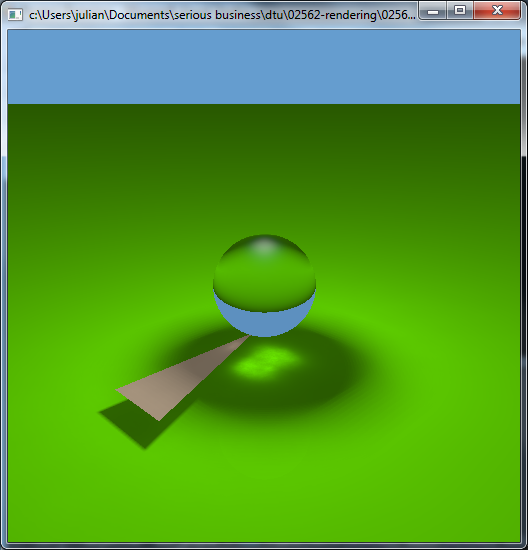
\includegraphics[width=8cm]{screenshots/project/04-caustic_map.png}
  \caption{Seperat \emph{caustic photon map}}
  \label{fig:caustic_photon_map}
\end{figure}

%%% Local Variables: 
%%% mode: latex
%%% TeX-master: "report_main"
%%% End: 
